\documentclass[11pt,a4paper,twoside,pdf]{article}

% Paquetes (añade otros si los necesitas):

\usepackage[T1]{fontenc}
\usepackage[utf8]{inputenc}


\usepackage[pdftex,final]{graphicx}
\bibliographystyle{plain} % We choose the "plain" reference style

% Style package
% Font Package (Palatino)
\usepackage{mathpazo}
% Packages for specific capabilities
\usepackage{rotating} % for text rotation in tables
\usepackage{multirow} % for multirow in tables
\usepackage{subcaption} % Modern package for subfigures
% Packages for specific symbols
\usepackage{amssymb}
\usepackage{amsmath}
\usepackage{amsfonts}
\usepackage{braket}
\usepackage{eurosym} % Euro symbol
\usepackage{bbding} % for \XSolidBrush
\usepackage{pifont} % for \ding{55} (a check mark)
\usepackage{macro}
\usepackage{slashed}
\usepackage{cite}

\usepackage{latexsym}
\usepackage{comment}
\usepackage{soul}
\usepackage{array}
%\usepackage{marvosym}
\usepackage{epsfig}
\usepackage{graphics}
\usepackage{amsfonts}
\usepackage{xspace}
\usepackage{color}
\usepackage{booktabs}
\usepackage{xtab}
\usepackage[colorlinks=true,urlcolor=blue,linkcolor=blue,citecolor=blue]{hyperref}
\numberwithin{equation}{section}


\linespread{1.05}

% TFG en inglés:
\usepackage[english]{babel} 
\addto\captionsenglish{\renewcommand{\chaptername}{}}

% TFG en español:
%\usepackage[spanish,es-nodecimaldot,es-tabla,es-lcroman,es-nosectiondot,es-noindentfirst]{babel}
%\renewcommand\spanishchaptername{}

% Formato de la página:
\usepackage{fancyhdr}
\usepackage[top=2.88cm,bottom=2.97cm,left=2.95cm,right=2.95cm]{geometry}
\setlength{\parskip}{0.1cm}

% Pon aquí tus definiciones:

\newcommand{\dis}{\displaystyle}
%\sodef\an{}{.2em}{1em plus1em}{2em plus.1em minus.1em}

\begin{document}

% Portada %%%%%%%%%%%%%%%%%%%%%%%%%%%%%%%%%%%%%%%%%%%%%%%%%%%%%%%%%%%%%%%%%%%%%%

\pagestyle{empty}


\noindent
\begin{tabular}{r}

\includegraphics[width=8.8cm]{escudoUGRmonocromo.png} \\[-1.8ex]
\hspace{31mm}\vspace{-8mm}
\begin{tabular}{c}
\hline\\[-1ex]\hskip-2mm
{\bf Facultad de Ciencias}\hspace{18mm}
\end{tabular}
\end{tabular}

\large
\vspace{30mm}
\hspace{25mm}
\begin{tabular}{l}
GRADO EN F\'ISICA
\end{tabular}

\vspace{45mm}
\hspace{25mm}
\begin{tabular}{l}
TRABAJO FIN DE GRADO
\\[1.5ex]
\LARGE\bf Herramientas para cálculos \\ 
\LARGE\bf perturbativos en renormalización \\
\LARGE\bf de Hamiltonianos \\
\end{tabular}
%
\vfill
\hspace{25mm}
\begin{tabular}{l}
Presentado por:
\\
{\bf D. ZhuoZhuo Liu}
\\[3ex]
Curso Académico 2024/2025
\end{tabular}
%

\newpage
%
\begin{center}
{\bf Resumen}
\bigskip

\begin{minipage}{0.8\linewidth}
Los processos de renormalización son fundamentales para la comprensión de la 
teorías a distintas escalas, definiendo teorías efectivas que describen el
comportamiento de los sistemas para las distintas energías. Sin embargo, los 
cálculos son no triviales, y se emplean la teoría de perturbaciones para obtener
los resultados, representando los distintos términos de la teoría como diagramas 
que describen el proceso, similar a los diagramas de Feynman. Pero el número de
diagramas aumenta exponencialmente con el orden de la perturbación, haciendo que
el proceso de cálculo sea tedioso y propenso a errores. \\

El objetivo de este trabajo es desarrollar un programa que automatice el proceso
de obtención de los diagramas asociados a un proceso determinado, hasta un orden
dado, partiendo de unos diagramas base, llamado diagramas canónicos dados por la 
teoría. Siendo el programa capaz de descartar los diagramas que no contribuyen al 
proceso, detectar loops y añadir contratérminos a los diagramas para cancelar 
divergencias. \\

Analizando los diagramas obtenidos de ordenes inferiores, y comparando con 
resultados conocidos, se ha comprobado la veracidad del programa. Esto permite
obtener los diagramas de ordenes superiores, y estudiar el comportamiento de la 
teoría a dichos ordenes, en las que se pueden observar fenómenos único de teorías 
no abelianas.

\end{minipage}

\newpage

{\bf Abstract} 
\bigskip

\begin{minipage}{0.8\linewidth}
The renormalization procedure is fundamental to understand the behavior of the 
theories at different scales, defining effective theories that describe the
behaviour of the systems for different energy levels. However, the calculations are
non-trivial, and perturbation theory is used to obtain the results, representing
the different terms of the theory as diagrams that describe the process, similar
to the Feynman diagrams. But the number of diagrams increases exponentially with
the order of the perturbation, making the calculation process tedious and prone to
errors. \\

The aim of this work is to develop a program that automates the process of
obtaining the diagrams associated with a given process, up to a given order,
starting from a set of base diagrams, called canonical diagrams given by the
theory. The program is able to discard the diagrams that do not contribute to the
process, detect loops and add counterterms to the diagrams to cancel divergences. \\

By analysing the diagrams obtained from lower orders, and comparing with known
results, the correctness of the program has been verified. This allows to obtain
the diagrams of higher orders, and study the behavior of the theory at those
orders, where unique phenomena of non-abelian theories can be observed.

\end{minipage}

\newpage

\end{center}

% Indice %%%%%%%%%%%%%%%%%%%%%%%%%%%%%%%%%%%%%%%%%%%%%%%%%%%%%%%%%%%%%%%%%%%%%%%
%\newpage

\pagestyle{empty}       % no header (and no footer) on this page
\tableofcontents
\setcounter{page}{0}
\cleardoublepage        % finish the ToC

% Texto %%%%%%%%%%%%%%%%%%%%%%%%%%%%%%%%%%%%%%%%%%%%%%%%%%%%%%%%%%%%%%%%%%%%%%%%
%\newpage

\pagestyle{fancy}
\fancyhead[RO,LE]{\leftmark}
\fancyhead[LO,RE]{\thepage}
\fancyfoot{}

\newpage

\section{Introduction}

When trying to build a theory that describes the particles and their interactions, 
it's fundamental that the theory is compatible with the 2 pillars of modern physics,
the special relativity and quantum mechanics. The special relativity is a theory 
that's able to describe the behavior of particles at high energies, and quantum 
mechanics is a theory that describes the behavior of particles at small scales.
The combination of these two theories is the basis of the quantum field theory,
building a formalism that describes the particles as excitations of a field.

Other important aspect of the theory is that it should be able to describe the 
different phenomena that occur at different scales. In the context of QCD, the 
experiments performed at low energies, or high length scales, smear the interaction
between the particles, and does not resolve the details of the structure inside the
particles, observing strongly bound states. While at high energies, or low length 
scales, the hadrons are broken into their constituents, quarks and gluons, and the 
interaction between the particles is weak, forming the so-called asymptotic freedom.
The theory should be able to describe the transition between these two regimes.

In the context of theoretical physics, the renormalization group procedure is a 
powerful tool to study the behavior of physical systems at different scales. In
the case of quantum field theories, renormalization allows to study the system
at different energy scales by introducing a scale parameter, and by changing 
this parameter, the "resolution" of the system is changed, allowing to focus from 
the smallest details (the short distance behavior) to the largest ones (the grand 
scale behavior). 

We will adopt the Hamiltonian formalism to describe the dynamics of the system, 
working in the operator space, where the Hamiltonian operator governs the time
evolution of the states. 

Many widely used renormalization procedures tend to apply to Lagrangian dynamics. But 
in the framework of RGPEP, the renormalization group procedure is applied to 
Hamiltonian dynamics. The benefit of this approach is the ability obtain directly 
the solutions of the system (the spectrum of the theory, and the eigenstates of the 
Hamiltonian). RGPEP introduces an effective Hamiltonian, that describes the system at a
given scale. This effective Hamiltonian is the solution to a differential equation,
that describes the evolution of the effective Hamiltonian with respect to the
scale parameter.

In general, obtaining the exact solution of the RGPEP equation is a non-trivial task, 
and a perturbative expansion of the effective Hamiltonian is used to obtain the 
solution. By identifying each order in the Hamiltonian expansion with a series of 
products of diagrams, the next order in the expansion can be obtained from the 
diagrams of previous orders. Typically, these diagrams were analyzed hand, but the 
number of diagrams increases exponentially with each order, making the process 
tedious and error-prone. The goal of this thesis is to develop a code that automates 
the process of obtaining the diagrams associated with a certain interaction for a 
given order.

This thesis is organized as follows. Section \ref{sec:theoretical_background} describes
the theoretical background needed to understand the renormalization group procedure
for effective particles, and the Hamiltonian dynamics. Section \ref{sec:cases}
describes the case studied in this thesis, gluon self interactions, where
holding the simplicity of the scalar case, some peculiarities of the QCD theory are 
present. The section \ref{sec:code} describes the connection between the diagrams 
and the objects are defined in the code, as well as the steps taken to obtain higher 
order diagrams, that are presented in the section \ref{sec:diagrams}. Finally, the 
section \ref{sec:conclusions} presents the conclusions, future work and the 
improvement that can be done to the code.

\section{Theoretical background} \label{sec:theoretical_background}

To understand the basis of the RGPEP, we need to understand the different
concepts involved in the process, as well as the theories that the process is
applied to.  

\subsection{Fock space} \label{sec:fock_space}

Intoduced by V.A. Fock in 1932 \cite{1932ZPhy...75..622F}, the Fock space is a sum 
of a set of Hilbert spaces, each one corresponding to a different number of 
particles in the system. So in order to describe a variable number of particles in our 
system, the use of the Fock space is needed.

The Fock space is defined as the direct sum of tensor products of the single 
particle Hilbert space $\mathbb{H}$,

\begin{comment}
    \begin{equation}
    \mathbb{F}_\nu = \bigoplus_{n=0}^{\infty} S_\nu \mathbb{H}^{\otimes n} = 
    \mathbb{C} \oplus \mathbb{H} \oplus S_\nu(\mathbb{H} \otimes \mathbb{H}) 
    \oplus S_\nu(\mathbb{H} \otimes \mathbb{H}\otimes \mathbb{H}) \oplus \cdots,
\end{equation}
where $S_\nu$ is the symmetrization operator depending on whether the particles described
are bosonic or fermionic, it symmetrizes or antisymmetrizes the tensors, and 
$\mathbb{C}$ is the complex scalar, corresponding to the states with no particles.
\end{comment}

\begin{equation}
    \mathbb{F} = \bigoplus_{n=0}^{\infty}  \mathbb{H}^{\otimes n} = 
    \mathbb{C} \oplus \mathbb{H} \oplus (\mathbb{H} \otimes \mathbb{H}) 
    \oplus (\mathbb{H} \otimes \mathbb{H}\otimes \mathbb{H}) \oplus \cdots,
\end{equation}
where $\mathbb{C}$ is the complex scalar, corresponding to the states with no particles.

This way a general state in the Fock space can be expressed as,

\begin{equation}
    \ket{\Psi} = \ket{\Psi_0} \oplus \ket{\Psi_1} \oplus
    \ket{\Psi_2} \oplus \cdots = c \ket{0} + \sum_{i=1}c_i \ket{\psi_i} +
    \sum_{i,j=1}c_{ij} \ket{\psi_i \psi_j} + \cdots,
\end{equation}

where $\ket{\Psi_0}$ is the vacuum state, $\ket{\Psi_1}$ is the one particle
state, $\ket{\Psi_2}$ is the two particle state, and so on. The coefficients $a_i$
are the amplitudes of the states, in general complex numbers. 

In the case of QCD, a general state in the Fock space involves a superposition of all 
possible multiparticle states, build from quarks, antiquarks, and gluons, with the
correct quantum numbers. For instance, a quarkonium state in QCD is given by:

\begin{equation}
    \ket{\Psi} = c_1 \ket{q\bar{q}} + c_2 \ket{q\bar{q}g} + c_3 \ket{qqq} 
    + c_4 \ket{gg} + \cdots,
\end{equation}

\subsection{Hamiltonian dynamics}

In quantum field theory, 2 equivalent formulations of the dynamics can be used, 
the Lagrangian and the Hamiltonian formulations. Though the modeling of dynamics 
tends to start in the Lagrangian formulation, and then using the Legendre transformation
to obtain the Hamiltonian formulation. 

\subsubsection{Canonical Hamiltonian}\label{sec:canonical_hamiltonian}

\begin{comment}
\subsubsection{Classical mechanics}

The canonical Hamiltonian is a function of the canonical coordinates $q_i$,
the canonical momenta $p_i$, and time $t$. The Hamiltonian is a function that
describes the total energy of the system, and is obtained from applying the Legendre 
transformation to the Lagrangian of the system, this is defined as,
\begin{equation}
    H(q,p,t) = \sum_i p_i \dot{q}_i - L(q,\dot{q},t),
\end{equation}
where $H$ is the Hamiltonian, $L$ is the Lagrangian, $q_i$ are the canonical
coordinates, $\dot{q}_i$ are the canonical velocities, and $p_i$ are the
canonical momenta. The canonical momenta are defined as,
\begin{equation}
    p_i = \frac{\partial L}{\partial \dot{q}_i},
\end{equation}

The canonical Hamiltonian governs the time evolution of the system via the 
Hamilton equations of motion, which are given by,
\begin{equation}
    \dot{q}_i = \frac{\partial H}{\partial p_i}, \quad \dot{p}_i = -\frac{\partial H}{\partial q_i}.
\end{equation}

\subsubsection{Field theory}

In the case of field theories, a Hamiltonian density can be defined such that 
integrating over space coordinates the Hamiltonian is obtained. 

\begin{equation}
    H = \int d^3x \mathcal{H},
\end{equation}
for simplicity we will call the Hamiltonian density $\mathcal{H}$, as Hamiltonian.

For a classical field $\phi(x)$, with the Lagrangian density $\mathcal{L}
(\phi,\partial_\mu\phi)$, the Hamiltonian density is defined as,

\begin{equation}
    \mathcal{H} = \pi \dot{\phi} - \mathcal{L},
\end{equation}
where $\pi$ is the canonical momentum, defined as,

\begin{equation}
    \pi = \frac{\partial \mathcal{L}}{\partial \dot{\phi}}.
\end{equation}
\end{comment}

\begin{comment}
    

\subsubsection{Quantum field theory}

In quantum mechanics, or quantum field theory, the Hamiltonian becomes an operator 
acting on a Hilbert space. 

Solving the system means obtaining the spectrum of the theory, this is finding the 
eigenenergies of the system. In general this is a non trivial process. 

In field theory calculations the fundamental quantities to consider are the 
energy-momenta, angular momentum, and boosts, due to its symmetries
under the Poincaré group.

The Poincaré group contains the Lorentz group and the translations, the generators of
the Poincaré group are the four-momentum operator $P^\mu$ and the angular momentum
$M^{\mu\nu}$, which satisfy the following commutation relations,
\begin{align}
    \sbrackets{P^\mu, P^\nu} &= 0, \\
    \sbrackets{M^{\mu\nu}, P^\rho} &= 
    i\left( g^{\nu\rho}P^\mu - g^{\mu\rho}P^\nu \right), \\
    \sbrackets{M^{\mu\nu}, M^{\rho\sigma}} &    = i\left( g^{\nu\rho}M^{\mu\sigma} 
    - g^{\mu\rho}M^{\nu\sigma} + g^{\sigma\mu}M^{\nu\rho} - g^{\sigma\nu}
    M^{\mu\rho}\right).
\end{align}

\end{comment}

Consider a general field theory and a Lagrangian density 
$\mathcal{L}(\phi_a (x),\partial_\mu\phi_a (x))$\footnote{where $x$ indicate a 
4-vector, with $x^\mu$ its components, and $\partial_\mu = \frac{\partial}
{\partial x^\mu}$}, where $\phi_a (x)$ is a particular field of the system.
To obtain the Hamiltonian formulation, we need to define the 
canonical momenta,

\begin{equation}
    \pi_a (x) = \frac{\partial \mathcal{L}}{\partial (\partial_0 \phi_a (x))}.
\end{equation}

The Hamiltonian density, using the Legendre transformation,

\begin{equation}
    \mathcal{H} = \sum_a \pi_a (x) \partial_0 \phi_a (x) - 
    \mathcal{L}(\phi_a (x),\partial_\mu\phi_a (x)).
\end{equation}

In quantum mechanics, or quantum field theory, the Hamiltonian becomes an operator 
acting on a Hilbert space. This promotion of the Hamiltonian to an operator is done by
replacing the canonical coordinates and momenta with the corresponding operators, 
and impose the canonical commutation relations,

\begin{equation}
    \sbrackets{\phi_a (x), \pi_b (y)} = i \delta_{ab} \delta^3(x-y),
    \quad \sbrackets{\phi_a (x), \phi_b (y)} = 0, \quad
    \sbrackets{\pi_a (x), \pi_b (y)} = 0.
\end{equation}

The field operators tend to be expressed in terms of creation, $a_i$ and annihilation 
$a^\dagger_i$ operators, that act on the Fock space, creating and annihilating the mode 
$i$ of the field. Mathematically, the creation and annihilation operators are the 
Fourier components of the field.

Any state component in the Fock space can be expressed as the action of a series of 
creation operators on the vacuum state, $\ket{0}$,

\begin{equation}
    \ket{\Psi_n} = \sum_{i_1,i_2,\cdots,i_n} \frac{c_{i_1 i_2 \cdots i_n}}{\sqrt{n!}}
    a^\dagger_{i_1} a^\dagger_{i_2} \cdots a^\dagger_{i_n} \ket{0},
\end{equation}
making the full state, 

\begin{equation}
    \ket{\Psi} = \sum_{n=0}^{\infty} \frac{1}{\sqrt{n!}} \sum_{i_1,i_2,\cdots,i_n} 
    c_{i_1 i_2 \cdots i_n} a^\dagger_{i_1} a^\dagger_{i_2} \cdots a^\dagger_{i_n} \ket{0}.
\end{equation}

The creation and annihilation operators satisfy some commutation or anticommutation 
relations, depending on the nature of the particles, bosons or fermions. 

For bosons, the creation and annihilation operators satisfy the following commutation 
relations,

\begin{equation}
    \sbrackets{a_i, a_j^\dagger} = \delta_{ij}, \quad
    \sbrackets{a_i, a_j} = 0, \quad
    \sbrackets{a_i^\dagger, a_j^\dagger} = 0.
\end{equation}

For fermions, the creation and annihilation operators satisfy the following anticommutation
relations,

\begin{equation}
    \{a_i, a_j^\dagger\} = \delta_{ij}, \quad
    \{a_i, a_j\} = 0, \quad
    \{a_i^\dagger, a_j^\dagger\} = 0.
\end{equation}

This way, the creation and annihilation operators are the fundamental objects of the
Fock space, and the Hamiltonian and the fields are expressed in terms of these operators.


When a combination of creation and annihilation operators is considered, normal-ordering is
used when defining operators that contain both creation and annihilation operators
and avoid the infinite vacuum contribution. The normal-ordering is defined as the 
process of rearranging the creation and annihilation operators in such a way that 
all the creation operators are to the left of all the annihilation operators.

The normal-ordering is denoted by the symbol $:\cdots:$, then for a fermionic case, 

\begin{equation}
    a_i a_j^\dagger =  \{a_i, a_j^\dagger\} -  a_j^\dagger a_i = 
    \delta_{ij} - :a_j^\dagger a_i: = \delta_{ij} - a_j^\dagger a_i.
\end{equation}

\subsubsection{Front form of Hamiltonian Dynamics}


The quantization of the system is usually performed in the instant form of the 
dynamics, where the time is treated as the evolution parameter, and the rest of
coordinates are treated as spatial coordinates. But other forms of dynamics 
can be considered.

The front form (FF) or light front of dynamics introduced by Dirac (1949) 
\cite{dirac_front_forms_1949} offers a couple advantages to the instant form of 
dynamics typically considered in quantum field theory. 

Considering a quantization hypersurface defined by the equation,

\begin{equation}
    x^+ = \frac{1}{\sqrt{2}} (t+z) = \frac{1}{\sqrt{2}} (x^0 + x^3) = 0,
\end{equation}
then the rest of coordinates will be defined as

\begin{equation}
    x^- = \frac{1}{\sqrt{2}} (x^0-x^3), \quad x^\perp = (x^1, x^2),
\end{equation}

In the FF quantization, the space-time coordinate $x^+$ is treated as the evolution 
parameter, similar to the time parameter in the instant form, and the rest of 
coordinates, $x^-$ and $x^\perp$, are treated as spatial coordinates.

The Hamiltonian in FF quantization is obtained from the Lagrangian density using 
the Legendre transformation, similar to the procedure explained in the section
\ref{sec:canonical_hamiltonian}, but with respect to the new coordinates.

Describing the system in the FF quantization, the vacuum state is "empty", since 
no particle creation are possible from $P^+ = 0$

\subsection{RGPEP}
The RGPEP, is a renormalization group procedure applied to the Hamiltonian 
formulation. By considering a series of unitary transformations, the RGPEP is able to construct a 
series of effective Hamiltonians $\mathcal{H}_s$, and the corresponding effective 
particles, by the use of effective particle operators (namely creation and 
annihilation operators) that differs from the canonical ones by the unitary 
transformation $\mathcal{U}_s$,

\begin{equation}
    a_s = \mathcal{U}_sa_0\mathcal{U}_s^\dagger,
    \label{eq:effective_particle_operator}
\end{equation}
labeled by the parameter $s$, and is associated with the renormalization group scale
$\lambda = 1/s$. This parameter which has dimension of length, physically has the 
interpretation of the characteristic size of the effective particles.

Due to dimensional and notational reasons, it's convenient to consider the scale 
parameter $t = s^4$.

Then $s=0$ correspond to the point-like or bare particles, and recovering the 
original Hamiltonian $\mathcal{H}_0(a_0)$.

The effective Hamiltonian is related to the regulated canonical one with counter-terms 
by the condition,

\begin{equation}
    \mathcal{H}_t(a_t) = \mathcal{H}_0(a_0)
\end{equation}

Combining with the equation \eqref{eq:effective_particle_operator}, and considering 
the parameter $t$ instead of $s$, the condition becomes,

\begin{equation}
    \mathcal{H}_t(a_0) = \mathcal{U}_t^\dagger\mathcal{H}_0(a_0) \mathcal{U}_t,
\end{equation}
differentiating with respect of $t$, 

\begin{equation}
    \mathcal{H}_t^\prime (a_0) \equiv \frac{d}{dt}\mathcal{H}_t(a_0) = 
    \sbrackets{-\mathcal{U}_t^\dagger \mathcal{U}_t^\prime, \mathcal{H}_t(a_0)} 
    = \sbrackets{\mathcal{G}_t(a_0), \mathcal{H}_t(a_0)},
\end{equation}
where $\mathcal{G}_t$ is the RGPEP generator. We will consider the generator 
from Ref. \cite{PEP}

\begin{equation}
    \mathcal{G}_t = \sbrackets{\mathcal{H}_f, \mathcal{H}_{Pt}},
\end{equation}
where $\mathcal{H}_f$, the free part of $\mathcal{H}_t$, and $\mathcal{H}_{Pt}$ is 
defined as function of the interacting term. 

The free Hamiltonian $\mathcal{H}_f$ is the part of $\mathcal{H}_0(a_0)$ that does 
not depend on the coupling constants, 

This way, the RGPEP equation have the form,
\begin{equation}
    \mathcal{H}_t^\prime =  \sbrackets{\sbrackets{\mathcal{H}_f, \mathcal{H}_{Pt}}, \mathcal{H}_t},
\end{equation}

In general, the solution of the RGPEP equation is a non-trivial task, and a perturbative
expansion of the effective Hamiltonian is used to obtain the solution. Expressing  
$\mathcal{H}_t$ as a power series of the coupling constant $g$,

\begin{equation}
    \mathcal{H}_t = \sum_{n=0}^{\infty} g^n \mathcal{H}_{t n} = 
    \mathcal{H}_{0} + g \mathcal{H}_{t 1} + g^2 \mathcal{H}_{t 2} + g^3 \mathcal{H}_{t 3} +
    g^4 \mathcal{H}_{t 4} + \cdots.
\end{equation}

Plugging this expansion into the RGPEP equation, we obtain,
\begin{align}
    \begin{split}
    \mathcal{H}_{0}^\prime & + g \mathcal{H}_{t 1}^\prime  + g^2 \mathcal{H}_{t 2}^\prime
     + \cdots =  \\
     &= \sbrackets{\sbrackets{\mathcal{H}_0, \mathcal{H}_{0} + g \mathcal{H}_{Pt 1} 
     + g^2 \mathcal{H}_{Pt 2} + \cdots}, \mathcal{H}_{0} + g \mathcal{H}_{t 1} + g^2 \mathcal{H}_{t 2} + \cdots}. 
    \end{split}
\end{align}

Order by order in $g$, the following differential equations are obtained,
\begin{align}
        \mathcal{H}_{0}^\prime &= 0, \label{eq:diff_order0}\\
        g\mathcal{H}_{t 1}^\prime &= \sbrackets{\sbrackets{\mathcal{H}_0, g\mathcal{H}_{Pt 1}}, 
        \mathcal{H}_{0}}, \label{eq:diff_order1}\\
        g^2\mathcal{H}_{t 2}^\prime &= \sbrackets{\sbrackets{\mathcal{H}_0, g^2\mathcal{H}_{Pt 2}}, 
        \mathcal{H}_{0}} + \sbrackets{\sbrackets{\mathcal{H}_0, g\mathcal{H}_{Pt 1}}, 
        g\mathcal{H}_{t 1}}, \\
        g^3\mathcal{H}_{t 3}^\prime &= \sbrackets{\sbrackets{\mathcal{H}_0, g^3\mathcal{H}_{Pt 3}}, 
        \mathcal{H}_{0}} + \sbrackets{\sbrackets{\mathcal{H}_0, g^2\mathcal{H}_{Pt 2}}, 
        g\mathcal{H}_{t 1}} + \sbrackets{\sbrackets{\mathcal{H}_0, g\mathcal{H}_{Pt 1}}, 
        g^2\mathcal{H}_{t 2}}. \label{eq:diff_order3}\\
        &\vdots \nonumber
\end{align}

The order 0 term is solvable from a initial condition, and the solution will be a 
exponetial of the parameter $t$. The 1th order solution can be obtained from 0th 
order, and the 2nd order from the previous orders, and so on. 

\subsection{Regularization and Counterterms}

In QCD, the bare Hamiltonian is ill-defined due to the presence of elements 
that contain divergences, ultraviolet (UV) divergences and infrared (IR) divergences.
Th UV divergences are produced in processes where the large momentum transferes, 
or the high invariant mass difference between Fock states. While the IR divergences
are produced in procceses where the particles are "soft", carring small longitudinal
momentum fractions, $x_{p/P} = p^+/P^+$.

To deal with these divergences a regulating factor $r$ is 
introduced in the interacting terms. These factors make the interacting terms rapidly 
tend to zero, if the change in the transverse momentum of any gluon exceeds a certain
cutoff parameter $\Delta$, or if the change in longitudinal momentum of any gluon is
greater than a cutoff parameter $\delta$. 

The particle operators is multiplied by the regulating factor, 
\begin{equation}
    r_{\Delta \delta} (k^\perp, x) = r_\Delta (k^\perp) r_\delta(x) \theta(x).
\end{equation}

The transverse regulator factor will be of the form, 
\begin{equation}
    r_\Delta (\mathcal{M}) = \text{exp} \left( -\frac{\mathcal{M}^2}{\Delta^2} \right),
\end{equation}
with $\mathcal{M}$ the invariant mass of the system, ensuring that UV processes are
suppressed.

The longitudinal regulator factor must verify a similar condition, preventing terms
of the form $1/x$ or $1/x^2$ to blow up as x approaches 0. The exact form of the 
longitudinal regulator factor is not important, as long as it verifies the condition, 
since it will be removed using the RGPEP.

Both cutoff parameters will disappear in the final result, since the theory can't
depend on the cutoff parameters taken arbitrarily. This is done by taking the
limit $\Delta \to \infty$ and $\delta \to 0$, recovering the original values
taken by the momenta.

It's convenient to consider an abbreviated notation for the regulating factor, 
using the symbol $\tilde{r}_{P, p} = \tilde{r}_{\Delta \delta} (P,p)$, with,
\begin{equation}
    \tilde{r}_{\Delta \delta} (P,p) = r_{\Delta \delta} (p^\perp - x_{p/P}P^\perp) 
    r_{\Delta \delta}\sbrackets{P^\perp-p^\perp-\parenthesis{1-x_{p/P}}P^\perp, 1-x_{p/P}}.
\end{equation}

The counterterms is an additional term added to the initial or bare Hamiltonian 
$\mathcal{H}_0$ to deal with the divergences due to loops, produced during the 
process. This way, ensure that the effective Hamiltonian $\mathcal{H}_t$ remains 
finite at all values of $t$.

The counterterms are defined in a way, such that the coefficients of products 
of creation and annihilation operators in the effective theory for gluons of size $s$
become independent of the regularization parameter $\Delta$ when the regularization
in dynamics of gluons of size zero is being removed. The rest of the unknown parts 
of the counterterms are adjusted to respect the symmetries of the theory, and must 
match the predictions of the theory with the experimental results.

\subsection{Diagram representation}

From the expression of the Hamiltonian, different terms can be separated and correlate
to a diagram representation of the process. Each diagram will be composed of different elements, 

\begin{itemize}
    \item External legs, representation of the incoming and outgoing particles, it 
    indicates the type of process that is being considered. Will have different colors/
    types of lines depending on the type of particle.
    \item Internal legs, represent the virtual particles that are exchanged during the
    process, these particles are not observed in the final state. Similar to the
    external legs, will have different colors/types of lines depending on the type of
    particle.
    \item Vertices, points where interactions between particles occur, the number of
    vertices in a diagram indicates the order at which the diagram is contributing.
    \item Loops, closed paths in the diagrams, formed by the internal legs. It will
    indicate the presence of divergences in the process.
    \item Counterterms, additional terms added to the Hamiltonian to deal with the divergences
    produced during the process. These will be represented with a dot in the diagram.
\end{itemize}

Notice that the diagrams are similar to the Feynman diagrams, except for the presence
of the counterterms. The main difference is the order that the processes occur, altering
the order of the vertices in the diagram will produce a different process. 

Other difference how the diagrams are read, in the context of RGPEP, the diagrams are
read from the left to the right, meaning that the time evolution is from the left to 
the right.

As an example, consider the diagram in figure \ref{fig:example_diagram}, this pair of 
diagrams are one of the contributions to the 3 gluon vertex, with the counterterm 
associated with it. 

\begin{figure*}[h!]
    \centering
    \begin{subfigure}[t]{0.5\textwidth}
        \centering
        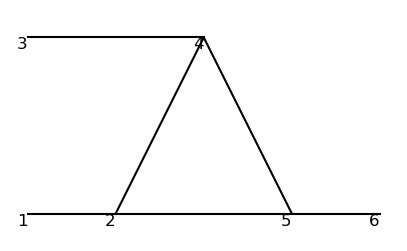
\includegraphics[width=0.7\textwidth]{plots/order3/order3_1to2/1.png}
        \caption{Diagram with a 3 gluon loop.}
    \end{subfigure}%
    \begin{subfigure}[t]{0.5\textwidth}
        \centering
        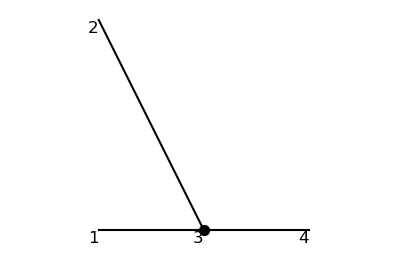
\includegraphics[width=0.7\textwidth]{plots/order3/order3_1to2/counterterms/1.png}
        \caption{Counterterm of the diagram}
    \end{subfigure}
    \caption{A example of a possible diagram, a third order contribution to the 
    process of 3 gluon vertex, 1 gluon incoming and 2 gluons outgoing. (Outputs of 
    the programs.)}
    \label{fig:example_diagram}
\end{figure*}

Following the previous definitions, the diagram represent a process where a gluon
interacts in a third order process, forming a 3 gluon loop, and 2 gluons are 
produced in the final state. Due to the presence of a loop, the diagram is
divergent, and a counterterm diagram is needed to deal with the divergence. This 
diagram is represented with a dot at the position of the loop, with the same 
external legs as the original diagram. 

\subsection{Order by order solutions.}

The solution of the differential equations \eqref{eq:diff_order1} to \eqref{eq:diff_order3} 
and so on, without considering the multiplicative factors, and relative phases between
the terms, can be expressed as,

\begin{align}
    \mathcal{H}_{t1} & = \mathcal{H}_{01} \\
    \mathcal{H}_{t2} & = \mathcal{G}_{02} + \mathcal{H}_{01} 
    \mathcal{H}_{01}\\
    \mathcal{H}_{t3} & = \mathcal{G}_{03} + \mathcal{H}_{01} \mathcal{H}_{01}
    \mathcal{H}_{01} + \parenthesis{\mathcal{G}_{02} \mathcal{H}_{01} + \mathcal{G}_{02}
    \mathcal{H}_{01} }\\
    \mathcal{H}_{t4} & = \mathcal{G}_{04} + \mathcal{H}_{01} \mathcal{H}_{01}
    \mathcal{H}_{01} \mathcal{H}_{01} + \parenthesis{\mathcal{G}_{02} 
    \mathcal{H}_{01} \mathcal{H}_{01} +  \mathcal{H}_{01} \mathcal{G}_{02}
    \mathcal{H}_{01} + \mathcal{H}_{01} \mathcal{H}_{01} \mathcal{G}_{02}} \nonumber\\
    & + \parenthesis{\mathcal{G}_{03} \mathcal{H}_{01} + \mathcal{H}_{01} 
    \mathcal{G}_{03} + \mathcal{G}_{02}\mathcal{G}_{02}}. \\
    &\vdots  \nonumber
\end{align}

This is an oversimplification of the solution, but it gives an idea of how the 
different solutions for each order are obtained. 

\section{Case study: Gluons self interactions} \label{sec:cases}

\subsection{Canonical Hamiltonian}

The Lagrangian density for the gluon fields is given by,
\begin{equation}
    \mathcal{L} = -\frac{1}{2}\text{tr}F^{\mu\nu}F_{\mu\nu},
\end{equation}
where $F^{\mu\nu}$ is the field strength tensor, defined as,
\begin{equation}
    F^{\mu\nu} = \partial^\mu A^\nu - \partial^\nu A^\mu + ig [A^\mu, A^\nu],
\end{equation}
and $A^\mu = A^{a\mu}t^a$, $t^a$ are the generators of the gauge group, and $g$ is the
coupling constant. Verifying the following relations,

\begin{equation}
    [t^a, t^b] = i f^{abc} t^c, \quad \text{tr}(t^a t^b) = \frac{1}{2} \delta^{ab}.
\end{equation}

We will be working in the gauge $A^+=0$, where the Lagrange equations constrain
the component $A^-$ to become 

\begin{equation}
    A^- = \frac{1}{\partial^+}2 \partial^\perp A^\perp - \frac{2}{\partial^{+2}} ig 
    \sbrackets{\partial^+ A^\perp, A^\perp}.
\end{equation}

In this way, the only degree of freedom left is the transverse component $A^\perp$.

As for the associated energy-momentum tensor,

\begin{equation}
    \mathcal{T}^{\mu\nu} = -F^{a\mu\alpha}\partial^\nu A^a_\alpha + 
    \frac{1}{4}g^{\mu\nu}F^{\alpha\beta} F_{\alpha\beta}.
\end{equation}

The Hamiltonian in FF quantization is obtained from integrating the component
$\mathcal{T}^{+-}$ of the energy-momentum tensor, over the hyperplane $x^+=0$. 

By working in the gauge $A^+=0$, the Hamiltonian density can be expressed as the sum of 
4 terms, as denoted in \cite{glazek_dynamics_2001}

\begin{equation}
    \mathcal{T}^{+-} = \mathcal{H}_{A^2} + \mathcal{H}_{A^3} +
    \mathcal{H}_{A^4} + \mathcal{H}_{[\partial AA]^2},
\end{equation}
with each of the terms, 

\begin{align}
    \mathcal{H}_{A^2} &= -\frac{1}{2} A^{\perp a} (\partial^\perp)^2 A^{\perp a}, \\
    \mathcal{H}_{A^3} &= g i \partial_\alpha A^a_\beta \sbrackets{A^\alpha, A^\beta}^a, \\
    \mathcal{H}_{A^4} &= -\frac{1}{4} g^2 \sbrackets{A_\alpha, A_\beta}^a
    \sbrackets{A^\alpha, A^\beta}^a, \\
    \mathcal{H}_{[\partial AA]^2} &= -\frac{1}{2} g^2 \sbrackets{i \partial^+ A^\perp,
    A^\perp}^a  \frac{1}{(i\partial^+)^2} \sbrackets{i\partial^+ A^\perp, A^\perp}^a.
\end{align}

Replacing $A^\mu$ with the operator $\hat{A}^\mu(x)$, defined by its Fourier composition
on the plane $x^+=0$,
\begin{equation}
    \hat{A}^\mu(x) = \sum _{\sigma c} \int [k] \sbrackets{t^c \epsilon^\mu_{k \sigma} 
    a_{k\sigma c}  e^{-ikx} + t^c \epsilon^{\mu*}_{k \sigma} 
    a^\dagger_{k\sigma c}  e^{ikx}}_{x^+=0},
\end{equation}
where $[k] = \theta(k^+) dk^+ d^2k^\perp / (16\pi^3k^+)$, $\epsilon^\mu_{k \sigma}$ 
are the polarization vectors, $t^c$ are the generators of the gauge group, and $a^\dagger_{k\sigma c}$, $a_{k\sigma c}$ are the 
creation and annihilation operators (particle operators), respectively. 


Substituting this expression into each term of the Hamiltonian densities, integrating
over space coordinates and taking into account the completeness and orthonormality 
of the polarization vectors, we obtain the following expression for the different
terms of the Hamiltonian \cite{QCDG}, 

\begin{align}
    H_{A^2} &= \sum_{\sigma c} \int [k] \frac{k^{\perp 2}}{k^+}a^\dagger_{k\sigma c}
    a_{k\sigma c}, \label{eq:H_A^2}\\
    H_{A^3} &= \sum_{123} \int [123] \slashed{\delta}(p^\dagger - p) \tilde{r}_{\Delta \delta}
    (3, 1) \sbrackets{gY_{123}a_1^\dagger a_2^\dagger a_3 + gY_{123}^*a_3^\dagger a_2 a_1},
    \label{eq:H_A^3}\\
    H_{A^4} &= \sum_{1234} \int [1234] \slashed{\delta}(p^\dagger - p) \frac{g^2}{4}
    \sbrackets{\parenthesis{\Xi_{A^4 1234} a_1^\dagger a_2^\dagger a_3^\dagger a_4 + h.c.}+ X_{A^4 1234} 
    a_1^\dagger a_2^\dagger a_3 a_4 }, \label{eq:H_A^4}\\
    H_{\sbrackets{\partial A A}^2} &= \sum_{1234} \int [1234] \slashed{\delta}
    (p^\dagger - p) g^2 \sbrackets{\parenthesis{\Xi_{\sbrackets{\partial A A}^2 1234}
    a_1^\dagger a_2^\dagger a_3^\dagger a_4 + h.c.} + X_{\sbrackets{\partial A A}^2 
    1234} a_1^\dagger a_2^\dagger a_3 a_4 } \label{eq:H_partial}.
\end{align}

\subsection{Canonical diagrams}
The canonical diagrams are the diagrams that are obtained from the canonical
Hamiltonian, and are the starting point to obtain the diagrams of higher order.

Following the creation and annihilation operators in the different terms of the 
Hamiltonian, we can distinguish the different types of process that are being
considered. 

Staring from the term $H_{A^2}$ in equation \eqref{eq:H_A^2}, we can see that this 
a particle of certain momentum $k$ is annihilated and created, producing the same
particle. This corresponds to the kinetic term of the Hamiltonian, and the diagram 
will be a line with the same color/type of particle in both ends. Being an order 0
term that will not contribute to the perturbative expansion.

The term $H_{A^3}$ in equation \eqref{eq:H_A^3} is a 3 gluon vertex, where either
1 gluon is annihilated and 2 gluons are created, or 2 gluons are annihilated, and
1 gluon is created. This process can be represented by a diagram with 3 external
legs, and 1 vertex. Being a order 1 term, with the corresponding diagrams shown in
figure \ref{fig:cannonical1}.

\begin{figure*}[h!]
    \centering
    \begin{subfigure}[t]{0.33\textwidth}
        \centering
        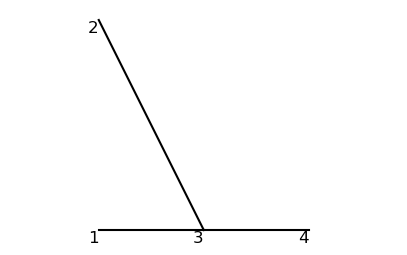
\includegraphics[width=\textwidth]{plots/canonical/order1/1.png}
        \caption{ }
    \end{subfigure}%
    \begin{subfigure}[t]{0.33\textwidth}
        \centering
        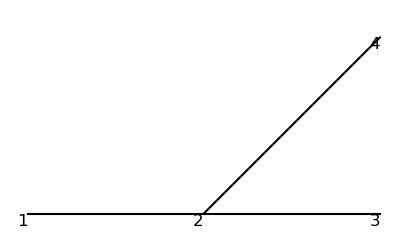
\includegraphics[width=\textwidth]{plots/canonical/order1/2.png}
        \caption{ }
    \end{subfigure}
    \caption{Canonical diagrams of order 1}
    \label{fig:cannonical1}
\end{figure*}

The term $H_{A^4}$ in equation \eqref{eq:H_A^4} is a 4 gluon vertex, where either
1 gluon is annihilated, and 3 gluons are created, 3 gluons are annihilated, and
1 gluon is created, or 2 gluons are annihilated, and 2 gluons are created. But we 
will not pay special attention to this term, since all the possible diagrams can be 
created from the diagrams of order 1.

The really interesting term is the term $H_{\sbrackets{\partial A A}^2}$ in
equation \eqref{eq:H_partial}, similar to the term $H_{A^4}$, this term is a 4 gluon
vertex, but the concept of instantaneous interaction is introduced. This allows to 
consider processes where a gluon is annihilated, and 3 gluons are created, to a 
pair of 3 gluon vertices. This process is usually represented in by a perpendicular
bar in the line of the gluon, indicating that the interaction is instantaneous, 
but due to program limitations, dotted lines are used in this work.

The different sum terms in the equation \eqref{eq:H_partial} indicate the different 
processes that can be considered, the first term $\Xi_{\sbrackets{\partial A A}^2 1234}$
indicate the process where 1 gluon is annihilated, and 3 gluons are created, as shown in
figure \ref{fig:cannonical2_1to3}. The second term $\Xi_{\sbrackets{\partial A A}^2 1234}^*$
indicate the hermitian conjugate of the first term, where 3 gluons are annihilated, and
1 gluon is created, as shown in figure \ref{fig:cannonical2_3to1}. The third term
$X_{\sbrackets{\partial A A}^2 1234}$ indicate the process where 2 gluons are annihilated,
and 2 gluons are created, as shown in figure \ref{fig:cannonical2_2to2}.

\begin{figure*}[h!]
    \centering
    \begin{subfigure}[t]{0.33\textwidth}
        \centering
        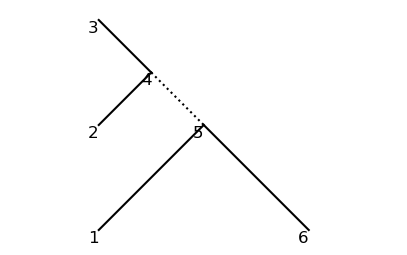
\includegraphics[width=\textwidth]{plots/canonical/order2/1.png}
        \caption{ }
    \end{subfigure}%
    \begin{subfigure}[t]{0.33\textwidth}
        \centering
        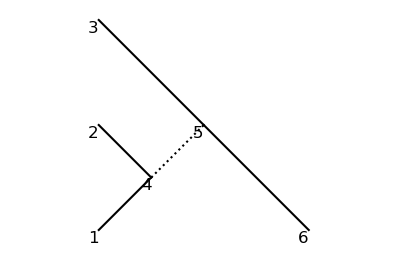
\includegraphics[width=\textwidth]{plots/canonical/order2/2.png}
        \caption{ }
    \end{subfigure}
    \begin{subfigure}[t]{0.33\textwidth}
        \centering
        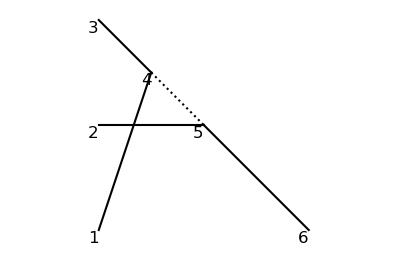
\includegraphics[width=\textwidth]{plots/canonical/order2/3.png}
        \caption{ }
    \end{subfigure}
    \caption{Canonical diagrams of order 2, for the term $\Xi_{\sbrackets{\partial AA}^2}$, 
    where one gluon is annihilated, and 3 gluons are created.}
    \label{fig:cannonical2_1to3}
\end{figure*}

\begin{figure*}[h!]
    \centering
    \begin{subfigure}[t]{0.33\textwidth}
        \centering
        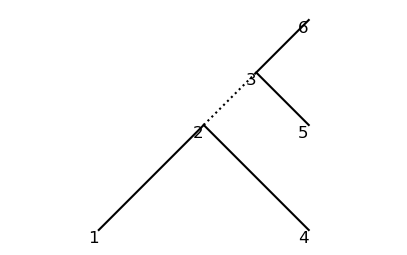
\includegraphics[width=\textwidth]{plots/canonical/order2/9.png}
        \caption{ }
    \end{subfigure}%
    \begin{subfigure}[t]{0.33\textwidth}
        \centering
        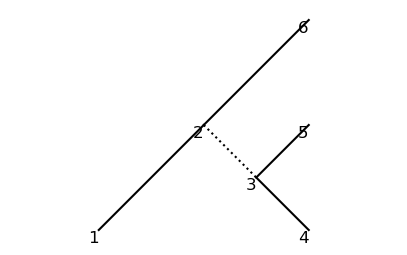
\includegraphics[width=\textwidth]{plots/canonical/order2/10.png}
        \caption{ }
    \end{subfigure}
    \begin{subfigure}[t]{0.33\textwidth}
        \centering
        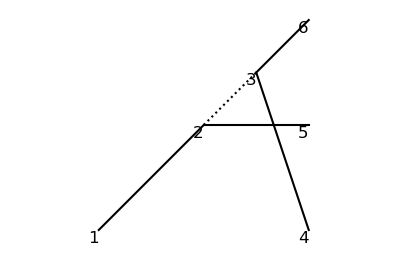
\includegraphics[width=\textwidth]{plots/canonical/order2/11.png}
        \caption{ }
    \end{subfigure}
    \caption{Canonical diagrams of order 2, for the term hermitian conjugate of 
    $\Xi_{\sbrackets{\partial AA}^2}$, where 3 gluons are annihilated, and
    1 gluon is created.}
    \label{fig:cannonical2_3to1}
\end{figure*}

\begin{figure*}[h!]
    \centering
    \begin{subfigure}[t]{0.24\textwidth}
        \centering
        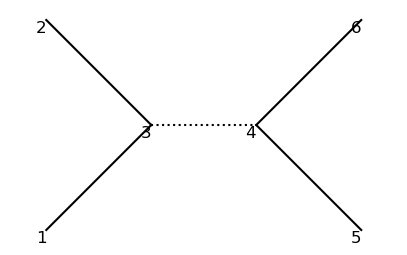
\includegraphics[width=\textwidth]{plots/canonical/order2/4.png}
        \caption{ }
    \end{subfigure}%
    \begin{subfigure}[t]{0.24\textwidth}
        \centering
        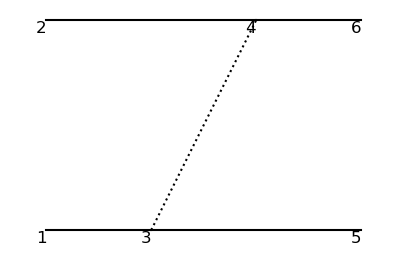
\includegraphics[width=\textwidth]{plots/canonical/order2/5.png}
        \caption{ }
    \end{subfigure}
    \begin{subfigure}[t]{0.24\textwidth}
        \centering
        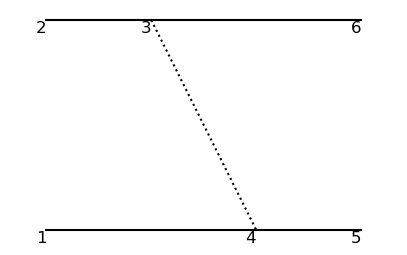
\includegraphics[width=\textwidth]{plots/canonical/order2/6.png}
        \caption{ }
    \end{subfigure}
    \begin{subfigure}[t]{0.24\textwidth}
        \centering
        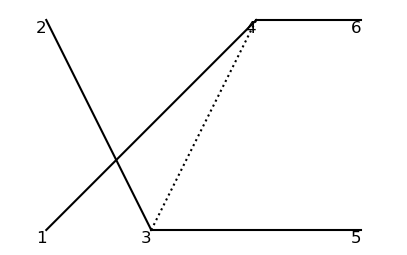
\includegraphics[width=\textwidth]{plots/canonical/order2/7.png}
        \caption{ }
    \end{subfigure}
    \begin{subfigure}[t]{0.24\textwidth}
        \centering
        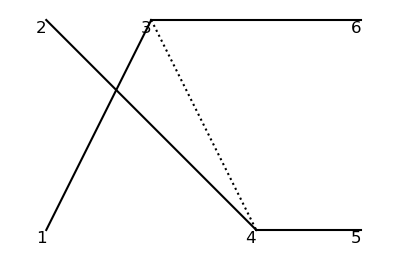
\includegraphics[width=\textwidth]{plots/canonical/order2/8.png}
        \caption{ }
    \end{subfigure}
    \caption{Canonical diagrams of order 2, for the term $X_{\sbrackets{\partial AA}^2}$, 
    where 2 gluons are annihilated, and 2 gluons are created.}
    \label{fig:cannonical2_2to2}
\end{figure*}

The combination of all these diagrams, are the canonical diagrams of order 2.
Together with the diagrams of order 1, figure \ref{fig:cannonical1},
they form the basis of the perturbative expansion of the Hamiltonian, and the
starting point to obtain the diagrams of higher order.

\newpage

\section{Code implementation} \label{sec:code}

The code is implemented in Python, but the general method can be applied to any 
programming language. The program is designed to be modular, and applicable to
other theories, by considering some minor modifications and changing the canonical
diagrams. These modifications are not implemented yet, and remain to be tested.

\subsection{Diagrams definition}

The diagrams are defined by 2 arrays, 
\begin{itemize}
    \item Points: arrays of dimension $N \times 2$, where $N$ is the number of 
    points in the diagram, each point is defined by its coordinates $(x,y)$.
    \item Paths: arrays of dimension $M \times N^\prime \times 2$, where $M$ is the
    number of different types of particles to consider in the theory, $N^\prime$ 
    is the number of paths for each types of particle in the diagram, and $2$ indicate
    the points to connect.
\end{itemize}

This way of defining the diagrams is analogous to the way of defining the undirected 
graphs in the graph theory, where the points are the vertices and the paths are the 
edges. 

In the case of gluon interactions, although only 1 type of particle is present, the
instantaneous interactions have to be considered. This is done by defining this 
interaction as a new type of virtual particle in the program.


\subsection{Order by order procedure}

To calculate the diagrams of higher order, the code follows the order by order 
procedure described in the section \ref{sec:theoretical_background}. Having only the
canonical diagrams, the program aims to obtain all the possible diagrams of an order
that contribute to a certain process, discarding the other diagrams.

This process produces a huge amount of diagrams, many of them equivalent. The 
program detects these repeated diagrams, and adds their contribution, thus reducing 
the number of diagrams that needs to be used to calculate the next order. This procedure
is the most time-consuming process of the program, needing a search algorithm to find
the equivalent diagrams, meaning that as the order increases, the number of diagrams
increases exponentially, and the time to find the equivalent diagrams increases
exponentially too. 

Although the process of finding the equivalent diagrams is time-consuming, it is
fundamental to reduce the global computational time. Since the number of diagrams 
tend to decrease by 1 to 2 orders of magnitude, depending on the order and the number of
particles in the process. This way reduces the time needed to calculate the
diagrams of the next order, so at the grand scale, the time needed to calculate
the diagrams of till a certain order is reduced by performing the search algorithm 
inbetewen the orders.

Other important aspect of the RGPEP are the counterterms, that are added to cancel 
the divergences produced in the process. The program is able to detect the 2 loops
and 3 loops in the diagrams of a certain order, and add new diagrams to cancel the 
divergences. As shown in figure \ref{fig:example_diagram}.




\section{Diagrams obtained} \label{sec:diagrams}


\subsection{Order 3}

Considering the 3 gluon vertex, the process of 1 gluon going to 2 gluons, up till 
order 3, the diagrams obtained from the program are shown in the figures 
\ref{fig:order3_1to2} and \ref{fig:order3_1to2/counterterms}.

\begin{figure*}[h!]
    \centering
    \begin{subfigure}[t]{0.24\textwidth}
        \centering
        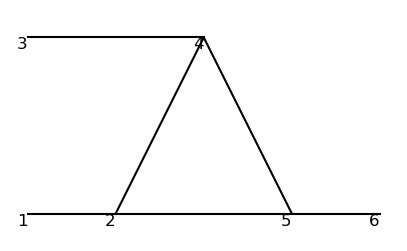
\includegraphics[width=\textwidth]{plots/order3/order3_1to2/1.png}
        \caption{ }
    \end{subfigure}%
    \hfill
    \begin{subfigure}[t]{0.24\textwidth}
        \centering
        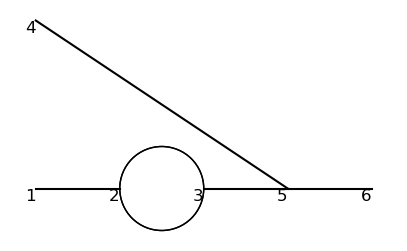
\includegraphics[width=\textwidth]{plots/order3/order3_1to2/2.png}
        \caption{ }
    \end{subfigure}
    \hfill
    \begin{subfigure}[t]{0.24\textwidth}
        \centering
        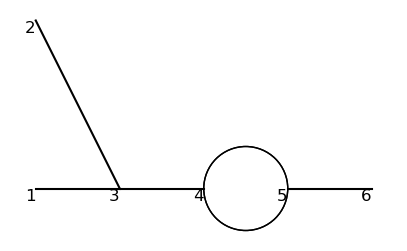
\includegraphics[width=\textwidth]{plots/order3/order3_1to2/3.png}
        \caption{ }
    \end{subfigure}
    \hfill
    \begin{subfigure}[t]{0.24\textwidth}
        \centering
        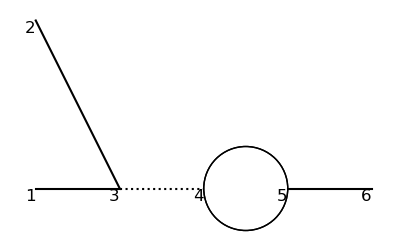
\includegraphics[width=\textwidth]{plots/order3/order3_1to2/4.png}
        \caption{ }
    \end{subfigure}
    \hfill
    \begin{subfigure}[t]{0.24\textwidth}
        \centering
        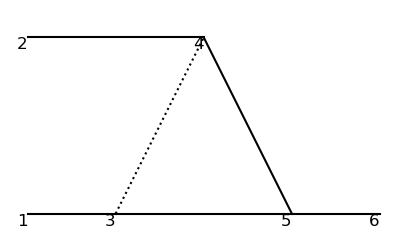
\includegraphics[width=\textwidth]{plots/order3/order3_1to2/5.png}
        \caption{ }
        \label{fig:order3_1to2/5}
    \end{subfigure}
    \hfill  
    \begin{subfigure}[t]{0.24\textwidth}
        \centering
        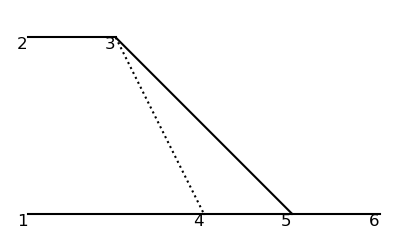
\includegraphics[width=\textwidth]{plots/order3/order3_1to2/6.png}
        \caption{ }
        \label{fig:order3_1to2/6}
    \end{subfigure}
    \hfill
    \begin{subfigure}[t]{0.24\textwidth}
        \centering
        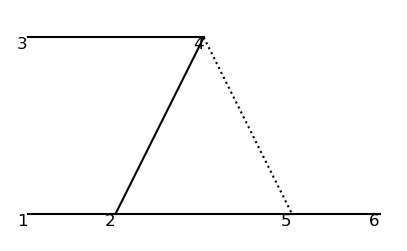
\includegraphics[width=\textwidth]{plots/order3/order3_1to2/7.png}
        \caption{ }
    \end{subfigure}
    \hfill 
    \begin{subfigure}[t]{0.24\textwidth}
        \centering
        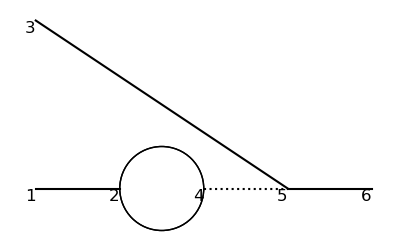
\includegraphics[width=\textwidth]{plots/order3/order3_1to2/8.png}
        \caption{ }
    \end{subfigure}
    \caption{Diagrams of third order, contributing to the 3 gluon vertex.}
    \label{fig:order3_1to2}
\end{figure*}

\begin{figure*}[h!]
    \centering
    \begin{subfigure}[t]{0.24\textwidth}
        \centering
        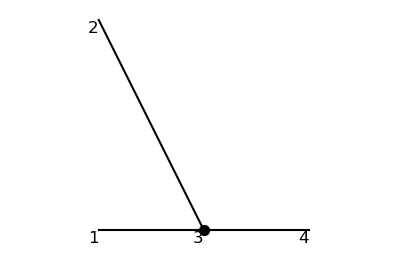
\includegraphics[width=\textwidth]{plots/order3/order3_1to2/counterterms/1.png}
        \caption{ }
    \end{subfigure}%
    \hfill
    \begin{subfigure}[t]{0.24\textwidth}
        \centering
        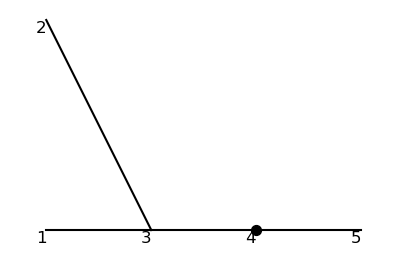
\includegraphics[width=\textwidth]{plots/order3/order3_1to2/counterterms/2.png}
        \caption{ }
    \end{subfigure}
    \hfill
    \begin{subfigure}[t]{0.24\textwidth}
        \centering
        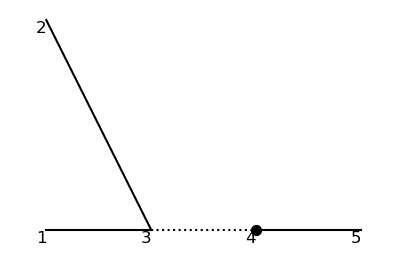
\includegraphics[width=\textwidth]{plots/order3/order3_1to2/counterterms/3.png}
        \caption{ }
    \end{subfigure}
    \hfill
    \begin{subfigure}[t]{0.24\textwidth}
        \centering
        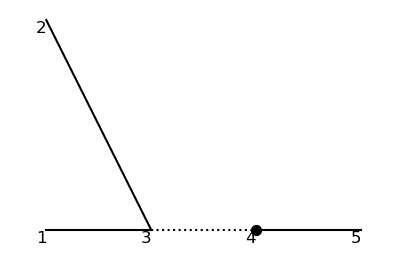
\includegraphics[width=\textwidth]{plots/order3/order3_1to2/counterterms/4.png}
        \caption{ }
        \label{fig:order3_1to2/counterterms/4}
    \end{subfigure}
    \hfill
    \begin{subfigure}[t]{0.24\textwidth}
        \centering
        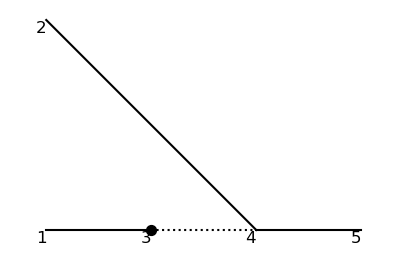
\includegraphics[width=\textwidth]{plots/order3/order3_1to2/counterterms/5.png}
        \caption{ }
        \label{fig:order3_1to2/counterterms/5}
    \end{subfigure}
    \caption{Counterterms to the diagrams of third order in figure \ref{fig:order3_1to2}}
    \label{fig:order3_1to2/counterterms}
\end{figure*}


In the figure \ref{fig:order3_1to2} we can see the diagrams obtained for the process
of 1 gluon going to 2 gluons, with the corresponding counterterms in figure
\ref{fig:order3_1to2/counterterms}. 

The diagrams \ref{fig:order3_1to2/5} and \ref{fig:order3_1to2/6} are really the same 
diagram, due to instant process being instantaneous. For any other particle, these 
2 diagrams would be different, due to the importance of the order in the interactions
so the program is kept to consider them as different, to not lose generality.

Other artifact of the program occur for the diagrams \ref{fig:order3_1to2/counterterms/4} and
\ref{fig:order3_1to2/counterterms/5}, which are counterterms added to cancel the divergences
in the canonical diagrams.

Comparing with the 3rd order contribution diagrams in \cite{QCDG}, the same diagrams
for the 3 gluon vertex are obtained, proving the validity of the program to reproduce the same results.



\subsection{Order 4}

Considering glueball states, the process of 2 gluons going to 2 gluons, the program
produces about 100 diagrams, with the corresponding counterterms. All the diagrams are
not shown here, since they are too many to be included in this document. But let's 
discuss some of the most interesting diagrams.

\begin{figure*}[h!]
    \centering
    \begin{subfigure}[t]{0.33\textwidth}
        \centering
        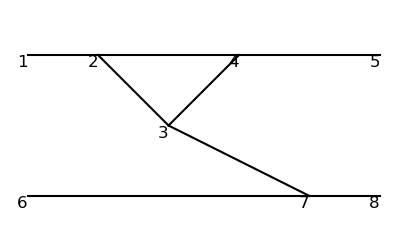
\includegraphics[width=\textwidth]{plots/order4/1.png}
        \caption{ }
    \end{subfigure}%
    \begin{subfigure}[t]{0.33\textwidth}
        \centering
        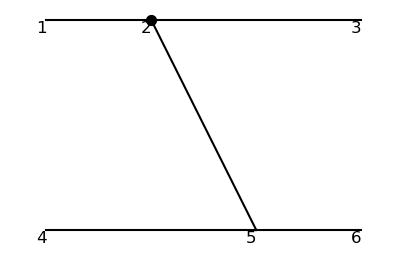
\includegraphics[width=\textwidth]{plots/order4/counterterms/1.png}
        \caption{ }
    \end{subfigure}
    \caption{Diagrams of fourth order, contributing to the 2 gluon vertex.}
    \label{fig:order4/1}
\end{figure*}

Starting at order 4, the distinct non-abelian nature of the QCD is present, since 
the gluons interact with themselves, creating diagrams not possible in abelian theories, 
such as QED. One of such processes is shown in the figure \ref{fig:order4/1}, where the


\subsection{Higher orders}

At higher orders, the diagrams become more complex, and the number of diagrams scale 
exponentially. Is here where the power of the program is shown. 

\begin{table} [h!]
    \centering
    \begin{tabular}{|c|c|c|}
        \hline
        Order & Unique diagrams & Computational time (s)\\
        \hline
        2  & 16 & 0.150\\
        3  & 76 & 0.198\\
        4  & 612 & 1.166\\
        5  & 5871  & 10.935\\
        6  & 65000  & 157.121\\
        \hline
    \end{tabular}
    \caption{Number of diagrams obtained by the program at each order, and the Computational
    time taken to calculate the diagrams.}
    \label{tab:diagrams}
\end{table}


\section{Conclusions and future work} \label{sec:conclusions}



% Referencias %%%%%%%%%%%%%%%%%%%%%%%%%%%%%%%%%%%%%%%%%%%%%%%%%%%%%%%%%%%%%%%%%
\newpage

\bibliography{references} % Entries are in the references.bib file

\end{document}

